\subsubsection{Caratteristiche di $ \R $}

\osservazione{
    \begin{itemize}
    \item $ \R $\marginnote{27 set 2021} non può essere messo in corrispondenza biunivoca con $ \N $.
    \item $ \R $ non è numerabile (mentre $ \N\leftrightarrow \Z\leftrightarrow \Q $ tutti numerabili).
    \item diciamo che gli insiemi in corrispondenza biunivoca tra di loro sono \textit{equipotenti}.
    \item Gli insiemi equipotenti a $ \N $ hanno \textit{potenza del numerabile}.
    \item Gli insiemi equipotenti ad $ \R $ hanno \textit{potenza del continuo}.
    \end{itemize}
}

Obiettivo: verifichiamo che in $ \R $ \[
    x^{2}=2
\] ammette soluzione (ovvero che esista la diagonale del quadrato di lato 1)

\teorema{jjillklucrezaibiosso}{
    Sia $ a \in \R $, $ a>0 $, allora \[
        \exists\, s \in \R, s>0\,\tc\, s^{2}=a.
    \]
}
\dimostrazione{jjillklucrezaibiosso}{
    \begin{itemize}
        \item Sia $ a>1 $ (ovvero $ a^{2}>a $), consideriamo \[
            A=\{x \in \R; x\ge 0\,\land\, x^{2}<a\}
        \]
        Verifichiamo che $ A $ è limitato superiormente da $ a $. Se così non fosse avremmo per assurdo \[
            \exists\, x \in A\,|\, x\ge a>1
        \] dunque \[
            x^{2}\ge a^{2}\ge a
        \] 
        
        $\implies$ $ \exists\, x \in A $ tale che $ x^{2}\ge a $, contraddizione. Allora per l'assioma $ \mathcal{R}_4 $ (completezza) \[
            \exists\, s =\sup A
        \]

        Verifichiamo che $ s^{2}=a $. Ragioniamo per assurdo: \[
            s^{2}\neq a: \begin{cases}
                s^{2}< a &(i)\\
                \lor\\
                s^{2}>a &(ii)
            \end{cases}
        \]
        \begin{itemize}
            \item [(\textit{i})] $ s^{2}<a$ applichiamo lo schema per assurdo \[
                s=\sup A \,\land \, s^{2}<a \,\implies\, s\neq \sup A
            \]
            Se troviamo $ \varepsilon>0 $ tale che $ (s+ \varepsilon)^{2}<a $ si ha $ (s+ \varepsilon) \in A $ ossia $ s \neq \sup A $, contraddizione. Cerchiamo tale $ \varepsilon $

            Osserviamo \[
                (s+ \varepsilon)^{2}=s^{2}+2s \varepsilon+ \varepsilon^{2}\le s^{2}+2s \varepsilon+ \varepsilon
            \] se $ 0< \varepsilon\le 1 $. Inoltre \[
                s^{2}+2s \varepsilon+ \varepsilon < a \,\iff\, s^{2}+ \varepsilon(2s+1)<a\,\iff\, 0< \varepsilon\le \frac{a-s^{2}}{2s+1}
            \]

            Consideriamo ora \[
                \varepsilon=\min \big\{1, \frac{a-s^{2}}{2s+1}\big\}
            \] si ha \[
                (s+ \varepsilon)^{2}=s^{2}+2s \varepsilon+ \varepsilon <a
            \] dunque $ (s+ \varepsilon)^{2}<a $ 
            
            $\implies$ $ \exists\, \varepsilon>0 $ tale che \[
                (s+ \varepsilon) \in A
            \] 
            
            $\implies$ $ s \neq \sup A $ contraddizione
        \item [(\textit{ii})] $ s^{2}>a $ se esistesse $ \varepsilon>0 $ tale che $ (s- \varepsilon)^{2}>a $ allora \[
            \forall\, x \in A\quad x^{2}<a<(s- \varepsilon)^{2}
        \] 
        
        $\implies$ $ \forall\, x \in A $, $ x<s- \varepsilon $, $ s \neq \sup A $. 

        Troviamo tale $ \varepsilon>0 $ \[
            (s- \varepsilon)^{2}=s^{2}-2s \varepsilon + \varepsilon^{2}> s^{2}-2 s \varepsilon
        \] ma \[
            s^{2}-2 s \varepsilon>a \,\iff\, s^{2}-a > 2s \varepsilon \,\iff\, 0< \varepsilon< \frac{s^{2}-a}{s_2}
        \]

        Concludiamo dicendo che \[
            \exists\, \varepsilon>0 \,\tc\, (s- \varepsilon)^{2}>a
        \] dunque $ s\neq \sup A $, contraddizione.
        \end{itemize}
        Punto della situazione: se $ a>1 $, allora $ s=\sup A $, si ha $ s^{2}=a $, dunque $ x^{2}=a $ ammette soluzione $ s=\sup A $.
        \item Sia $ a=1 $: la soluzione ovvia di $ x^{2}=1 $ è $ x=1 $
        \item Sia $ a<1 $.
        
        Sia $ b=1/a>1 $, allora esiste $ s=\sup\{x \in \R; x^{2}<b\} $ tale che $ s^{2}=b $, allora \[
            1/s^{2}=1/b=a
        \] 
        
        $\implies$ $ \exists\, R \in \R $ tale che $ R^{2}=a $.\qed
    \end{itemize}
}

\osservazione{
    Per cercare $ \varepsilon>0 $ tale che $ (s+ \varepsilon)^{2}<a $, $ a>1 $, $ s>0 $, $ s^{2}<a $, qualcuno avrebbe potuto pensare di svolgere i seguenti calcoli: \begin{multline*}
        (s+ \varepsilon)^{2}<a \,\iff\\
        \iff\, -\sqrt{a}< s+ \varepsilon < \sqrt{a}\,
        \iff\, -\sqrt{a}-s< \varepsilon<\sqrt{a}-s\,\iff\\\iff\, 0< \varepsilon< \sqrt{a}-s
    \end{multline*}

    Attenzione che la procedura è scorretta, in quanto $ \sqrt{a} $ non è stata ancora definita.
}

\definizione{}{
    In base al teorema precedentemente dimostrato possiamo affermare che: dato $ a>0 $, l'equazione \[
        x^{2}=a
    \] ammette un'unica soluzione positiva, precisamente \[
        s=\sup\{x \in \R, x^{2}<a, x>0\}
    \] indichiamo tale soluzione con $ \sqrt{a} $\begin{equation}
        \sqrt{a}=\sup\{x \in \R, x^{2}<a, x>0\}
    \end{equation}

    In generale, dato $ a>0 $, $ n \in \N\setminus \{0, 1\} $, $ \sqrt[n]{a} $ è l'unica soluzione positiva di $ x^{n}=a $
}

\teorema[(caratt. estremo superiore)]{carestrsupppspp}{
    Dato $ A \subseteq \R $
    
    \[S=\sup A\quad\iff\quad
    \begin{cases}
         \forall\, x \in A , \, x\le S \\
         \forall\, \varepsilon >0\quad\exists\, x \in A\,\tc\quad S- \varepsilon < x \le S
    \end{cases}
    \]
}
\dimostrazione{carestrsupppspp}{
    \begin{itemize}
        \item [``$\implies$''] Per assurdo sia la seconda implicazione falsa, ossia \[
            \exists\, \varepsilon>0\,|\, \forall\, x \in A\quad x\le S- \varepsilon
        \] allora $ S- \varepsilon < S $ è maggiorante di $ A $ 
        
        $\implies$ $ S\neq \sup A $ contraddizione.
        \item [``$\impliedby$''] Per assurdo sia $ S\neq \sup A $, allora esiste $ S' $ maggiorante di $ A $ con $ S'< S $.
        
        Poniamo $ \varepsilon=S-S' $ ($S'=S- \varepsilon$), allora abbiamo che \[
            \forall\, x \in A\quad x \le S' = S- \varepsilon
        \] e la seconda implicazione è negata: si ha contraddizione. \qed
    \end{itemize}
}

\teorema[(Densità di $ \Q $ in $ \R $)]{densqr}{
    \begin{equation}
        \forall\, a, b \in \R\quad \exists\, r \in \Q\,\tc\quad a<r<b
    \end{equation}
}

\subsection{Spazio Euclideo $ \R^{n} $}

Dato $ n \in \N\setminus\{0\} $, \[
    \R^{n}= \parentesi{n-\text{volte}}{\R\times \R \times\cdots\times \R}=\{x=(x_1, x_2, \cdots, x_{n} )\}
\]

\notazione{}{
    Scrivendo $ (a,b)$ conta l'ordine, in particolare \[
        (a,b)\neq (b,a).
    \]

    Scrivendo invece $ \{a,b\} $ non conta l'ordine, infatti \[
        \{a,b\}=\{b, a\}
    \]
}

\notazione{}{
    Il libro di testo spesso usa il grassetto per indicare gli elementi di $ \R^{n} $ \[
        \mathbf{x}=(x_1, \cdots, x_{n} )
    \]
    Altre notazioni \[
        \vec{x}=\overline{x}=(x_1, \cdots, x_{n} )
    \]

    Noi useremo \[
        x=(x_1, \cdots, x_{ne} )
    \]
}

\subsubsection{Operazioni su $ \R^{n} $}

\paragraph{Somma ($+$)}
\[
    \forall\, x, y \in \R^{n}\quad x+y=(x_1+y_1, \cdots, x_{n}+y_{n}  )
\]

In $ \R^{2} $ questa è la regola del parallelogramma
\proprieta[della somma]{La somma rispetta queste proprietà:

    $ \nu_{1} \hspace{0.2em} $$\left\{ %\{
	  \begin{minipage}{0.8\textwidth}
	    \begin{itemize}
            \item commutativa;
            \item associativa;
            \item esistenza dell'elemento neutro \[
                \underline{0}=(0,0,\cdots,0);
            \]
            \item esistenza dell'opposto: \[
                \forall\, x =(x_1, \cdots, x_{n} )
            \] $ x $ ammette opposto \[
                -x=(-x_1, -x_2, \cdots, -x_{n} )
            \] tale che $ x+(-x)=\underline{0} $.
        \end{itemize}
	  \end{minipage}\right.$
}

\paragraph{Prodotto per uno scalare $ \lambda \in \R $}
\[
    \forall\,x =(x_1, \cdots, x_{n} ) \in \R^{n}\quad \lambda \in \R
\] si definisce $ \lambda x $ come \[
    \lambda x=(\lambda x_1, \lambda x_2, \cdots, \lambda x_{n} )
\]

\proprieta[del prodotto]{
    $ \forall\, x, y \in \R^{n}$, $ \forall\, \lambda, \mu \in \R $ si ha che

    $ \nu_{2} \hspace{0.2em} $$\left\{ %\{
	  \begin{minipage}{0.8\textwidth}
	    \begin{itemize}
            \item $ \lambda(\mu \,x) = (\lambda\mu )x$;
            \item $ 1 \,x=x $;
            \item $ (\lambda+\mu)x=\lambda x + \mu x $;
            \item $ \lambda (x+y)= \lambda x +\lambda y $.
        \end{itemize}
	  \end{minipage}\right.$
}

$ \nu_{1}  $ e $ \nu_{2}  $ non saranno dimostrate.

Diciamo che $ \R^{n} $, dotato di somma e prodotto per scalare è uno \textit{spazio vettoriale} sullo scalare $ \R $.

\definizione{}{
    Dati \begin{align*}
        x &= (x_1, x_2, \cdots, x_{n} ) \in \R^{n}\\
        y &= (y_1, y_1, \cdots, y_{n} ) \in \R^{n}
    \end{align*} diciamo \textit{prodotto scalare} di $ x, y \in \R^{n} $ \begin{equation}
        \langle x, y\rangle :=\sum_{j=1}^{n} x_{j} y_{j}   
    \end{equation}
}
\attenzione{
    \begin{align*}
    \langle \bullet , \bullet  \rangle: \R^{n}\times \R^{n}& \to \R \\
    (x,y) & \mapsto \langle x, y\rangle
    \end{align*}
    Il prodotto scalare non è una operazione interna a $ \R^{n} $.
}
\proprieta[del prodotto scalare]{
    $ \forall\, x, y, z \in \R^{n} $, $ \forall\, \lambda \in \R $ si ha 

    $ \zeta \hspace{0.2em} $$\left\{ %\{
	  \begin{minipage}{0.8\textwidth}
	    \begin{enumerate}
        \item $ \langle x , x  \rangle\ge 0 $; $ \langle x , x  \rangle= 0\,\iff\, x=0 $;
        \item $ \langle x, y \rangle= \langle y, x \rangle $;
        \item $ \langle x+y, z \rangle = \langle x, z \rangle + \langle y, z \rangle$;
        \item $ \langle \lambda x, y \rangle = \lambda \langle x, y \rangle$
    \end{enumerate}
	  \end{minipage}\right.$

    Si dice che $ \langle \bullet , \bullet  \rangle $ è un'applicazione bilineare positiva da $ \R^{n}\times \R^{n}\to \R $
}

\esempio{}{
    \begin{align*}
        \vec{F} &=(f_1, f_2, f_3) \quad &\text{forza applicata ad un oggetto}\\
        \vec{x} &=(x_1, x_2, x_3) \quad &\text{spostamento}\\
        L &= \langle \vec{F}, \vec{x}\rangle \quad &\text{lavoro.}
    \end{align*}
}

\definizione{}{
    Dato $ x \in \R^{n} $ diciamo \textit{modulo} (norma) di $ x $ \begin{equation}
        |x|=\sqrt{\langle x, x\rangle}=\sqrt{\sum_{j=1}^{n}x_{j}^{2}  }.
    \end{equation}
}

\osservazione{
    \[
        |\bullet|: \R^{n}\to \R_{+}=\{a \in \R; a\ge 0\} 
    \] Risulta quindi che $ |-x|=|x| $.
}
\osservazione{}{
    In $ \R^{2} $, $ |x| $ rappresenta la lunghezza del vettore $ x $

    \begin{center}
        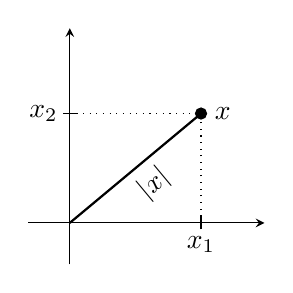
\begin{tikzpicture}% coordinates
            \begin{axis}[
                axis equal,
                axis lines=middle,
                no marks,
                xmin=-1,
                xmax=8,
                ymin=-1,
                ymax=8,
                enlargelimits, 
                scale only axis, 
                height=3cm, 
                width=3cm,
                xtick={0},
                ytick={0}
            ]
            \node [fill=white,anchor=center] at (6, -1) {$x_1$};
            \addplot [no marks, black ]coordinates {
				(6,-0.3)
                (6, 0.3)
			};
            \node [fill=white,anchor=center] at (-1.2, 5) {$x_2$};
            \addplot [no marks, black ]coordinates {
				(-0.3, 5)
                (0.3, 5)
			};
            \addplot [only marks, black ]coordinates {
				(6, 5)
			};
            \node [fill=white,anchor=center] at (7, 5) {$x$};
            \addplot [no marks, black, dotted ]coordinates {
				(6, 0)
                (6, 5)
			};
            \addplot [no marks, black, dotted ]coordinates {
				(0, 5)
                (6, 5)
			};
            \node [fill=white,anchor=center, rotate around={39.80:(0,0)}] at (3, 2.2) {$|x|$};
            \addplot [no marks, black, thick]coordinates {
				(0, 0)
                (6, 5)
			};
            
            \end{axis}
        \end{tikzpicture}
    \end{center}
    
Invece, per $ a \in \R $, \[
    |a|=\sqrt{a^{2}}=\begin{cases}
        a &a\ge 0\\
        -a & a<0
    \end{cases}
\] ovvero diventa equivalente al \textit{valore assoluto} di $ a $.
\begin{center}
    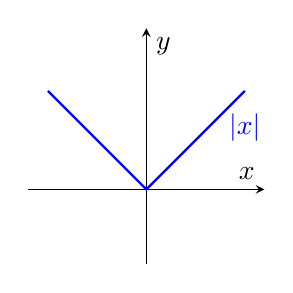
\begin{tikzpicture}% coordinates
        \begin{axis}[
            xlabel=$x$, 
            ylabel=$y$,
            axis equal,
            axis lines=middle,
            no marks,
            xmin=-8,
            xmax=8,
            ymin=-1,
            ymax=8,
            enlargelimits, 
            scale only axis, 
            height=3cm, 
            width=3cm,
            xtick={0},
            ytick={0}
        ]
        \node [fill=white,anchor=center] at (8, 5) {\textcolor{blue}{$|x|$}};
        \addplot [no marks, blue, thick] coordinates {
            (-8, 8)
            (0, 0)
            (8, 8)
        };
        \end{axis}
    \end{tikzpicture}
\end{center}
}

\proprieta[del modulo]{
    $ \forall\, x,y \in \R^{n} $, $ \forall\, \lambda, \mu \in \R $ si ha

    $ \eta \hspace{0.2em} $$\left\{ %\{
	  \begin{minipage}{0.8\textwidth}
	    \begin{enumerate}
            \item $|x|\ge 0; \quad |x|=0 \,\iff\, x=0    $    
            \item $|\lambda x| = |\lambda|\,|x|$
            \item $|x+y| \le |x|+ |y|$ (disuguaglianza triangolare)
        \end{enumerate}
	  \end{minipage}\right.$

    
}

\osservazione{
    \begin{align}
        |x|=|(x-y)+y|\le |x-y|+|y|\, &\iff\, |x|-|y|\le |x-y|\label{aaaaa}\\
        |y|=|(y-x)+x|\le |x-y|+|x| \,&\iff\, |x|-|y|\ge -|x-y|\label{bbbbb}
    \end{align}
    Mettendo insieme \eqref{aaaaa} e \eqref{bbbbb} otteniamo \[
        \forall\, x,y \in \R^{n}\quad -|x-y|\le |x|-|y|\le |x-y|
    \] da cui \begin{equation}
        \big| |x|-|y|\big| \le |x-y|
    \end{equation}
}

\nota{Ricordare che, dato $ a\ge 0 $, $ x \in \R $, \[
    |x|\le a \quad \iff\quad -a\le x\le a
\]}

\definizione{}{
    Dati $ x, y \in \R^{n} $ diciamo \textit{distanza} di $ x $ da $ y $\begin{equation}
        d(x,y):= |x-y|=\sqrt{\sum_{j=1}^{n}(x_{j}-y_{j})^{2} }
    \end{equation}
}

\proprieta[della distanza]{
    $ \forall\, x,y, z \in \R^{n} $ si ha 

    $ \mathcal{D} \hspace{0.2em} $$\left\{ %\{
	  \begin{minipage}{0.8\textwidth}
	    \begin{enumerate}
            \item $d(x,y)\ge 0;\quad d(x,y)=0\,\iff\, x=y$;
            \item $ d(x,y)=d(y,x)  $;
            \item $ d(x,y)\le d(x,z)+d(y,z)$ (disuguaglianza triangolare).
        \end{enumerate}
	  \end{minipage}\right.$
}

\definizione{}{
    $ \R^{n} $ e ogni altro insieme dotato di somma ($+$), prodotto per uno scalare e norma (distanza), sono detti \textit{spazi vettoriali normati} o \textit{spazi vettoriali metrici}.
}
